\documentclass[conference]{IEEEtran}
\IEEEoverridecommandlockouts
\usepackage[T1]{fontenc}
\usepackage{cite,amsmath,amssymb,graphicx,booktabs,array,url}
\usepackage{enumitem}
\newcounter{algorithm}
\usepackage{tikz}
\usetikzlibrary{arrows.meta,positioning}
\usepackage{etoolbox}
\makeatletter
\patchcmd{\abstract}{---}{: }{}{}
\patchcmd{\IEEEkeywords}{---}{: }{}{}
\makeatother
\usepackage[hidelinks]{hyperref}
\hypersetup{pdftitle={VeriFake: A TF-IDF and Ensemble Learning Framework for Web-Based Fake News Detection},pdfauthor={Md Mahbubur Rahman; Md. Abdur Rahman; Md. Hafizur Rahman Sumon; Shanta Islam; Md. Mahamudul Hasan; Md. Shahriar Alam Sakib; Md. Moudud Ahmmed; Ahmed Shafkat},pdfsubject={IEEE CSDE 2026, ieee-csde\_3824}}
\setlength{\emergencystretch}{1em}
\renewcommand{\topfraction}{0.9}
\renewcommand{\dbltopfraction}{0.9}
\renewcommand{\textfraction}{0.07}
\renewcommand{\floatpagefraction}{0.85}
\renewcommand{\dblfloatpagefraction}{0.85}
\setcounter{topnumber}{3}
\setcounter{dbltopnumber}{2}
\makeatletter
\newcommand{\linebreakand}{\end{@IEEEauthorhalign}\hfill\mbox{}\par\vspace{0.7\baselineskip}\mbox{}\hfill\begin{@IEEEauthorhalign}}
\makeatother
\begin{document}
\title{VeriFake: A TF-IDF and Ensemble Learning Framework for Web-Based Fake News Detection}
\author{\IEEEauthorblockN{Md Mahbubur Rahman}
\IEEEauthorblockA{\textit{Dept. of Electrical Engineering}\\\textit{and Computer Science}\\\textit{University of Wyoming}\\Laramie, WY 82071, USA\\mrahma11@uwyo.edu (corr.)}
\and
\IEEEauthorblockN{Md. Abdur Rahman}
\IEEEauthorblockA{\textit{Dept. of Computer Science}\\\textit{and Engineering}\\\textit{Dhaka International University}\\Satarkul, Dhaka-1213, Bangladesh}
\and
\IEEEauthorblockN{Md. Hafizur Rahman Sumon}
\IEEEauthorblockA{\textit{Dept. of Computer Science}\\\textit{and Engineering}\\\textit{Dhaka International University}\\Satarkul, Dhaka-1213, Bangladesh}
\linebreakand
\IEEEauthorblockN{Shanta Islam}
\IEEEauthorblockA{\textit{Dept. of Computer Science}\\\textit{and Engineering}\\\textit{Dhaka International University}\\Satarkul, Dhaka-1213, Bangladesh}
\and
\IEEEauthorblockN{Md. Mahamudul Hasan}
\IEEEauthorblockA{\textit{Dept. of Computer Science}\\\textit{and Engineering}\\\textit{Dhaka International University}\\Satarkul, Dhaka-1213, Bangladesh}
\and
\IEEEauthorblockN{Md. Shahriar Alam Sakib}
\IEEEauthorblockA{\textit{Dept. of Computer Science}\\\textit{and Engineering}\\\textit{Dhaka International University}\\Satarkul, Dhaka-1213, Bangladesh}
\linebreakand
\IEEEauthorblockN{Md. Moudud Ahmmed}
\IEEEauthorblockA{\textit{Dept. of Computer Science}\\\textit{and Engineering}\\\textit{Dhaka International University}\\Satarkul, Dhaka-1213, Bangladesh}
\and
\IEEEauthorblockN{Ahmed Shafkat}
\IEEEauthorblockA{\textit{Dept. of Electrical Engineering}\\\textit{and Computer Science}\\\textit{University of Wyoming}\\Laramie, WY 82071, USA}}
\IEEEpubid{\makebox[\columnwidth]{979-8-3195-4477-3/26/\$31.00~\copyright2026 IEEE\hfill}\hspace{\columnsep}\makebox[\columnwidth]{ }}
\maketitle
\IEEEpubidadjcol
\begin{tikzpicture}[remember picture,overlay]
\node[anchor=north east,align=right,font=\footnotesize,inner sep=0pt] at ([xshift=-0.62in,yshift=-0.28in]current page.north east)
{11th IEEE Asia-Pacific Conference on Computer Science and Data Engineering (IEEE CSDE 2026)\\1-3 November 2026, Cox's Bazar, Bangladesh};
\end{tikzpicture}

\begin{abstract}
VeriFake compares thirteen established classifiers using term frequency-inverse document frequency features and tests whether strong random-split performance survives author and dataset changes. After removing empty and repeated articles, the Kaggle collection contains 20,257 records. Feature fitting and hyperparameter selection use training data only. LinearSVC, selected by three-fold cross-validation Matthews correlation coefficient, achieves 98.15\% accuracy and 0.9630 Matthews correlation on 4,052 held-out articles. Accuracy is 96.80\% on a known-author-disjoint test, 71.49\% for Kaggle-to-ISOT transfer, and 58.47\% in reverse. Author-plus-title input reaches 99.56\% accuracy on the random split but 89.68\% under author separation. These gaps qualify apparently strong within-collection results. We document the evaluation procedure and a preprocessing-aware export for a Django prototype. VeriFake predicts dataset labels; it does not verify factual claims against external evidence.
\end{abstract}
\begin{IEEEkeywords}
fake news detection, TF-IDF, text classification, cross-dataset evaluation, author information, web application
\end{IEEEkeywords}

\section{Introduction}
News classifiers can learn author, topic, and publication-style cues that remain similar across a random split. High test accuracy then provides limited evidence of reliability on unfamiliar sources. Recent studies of dataset bias and out-of-distribution evaluation make this distinction explicit \cite{kishi,verhoeven}.

VeriFake compares thirteen classifiers using title-and-body TF-IDF. Ensemble learning in the title refers to the evaluated forests and boosting methods; no new architecture is proposed. The Django interface accepts news text and returns dataset-label predictions.

The contributions are a shared comparison with training-only feature fitting and Matthews correlation coefficient (MCC) selection; known-author-disjoint evaluation, bidirectional Kaggle/ISOT transfer, and author/title/body ablation; and a documented evaluation procedure with preprocessing-aware export. The central finding is the gap between within-collection accuracy and transfer.

\section{Related Work}
Zhou and Zafarani distinguish detection based on knowledge, writing style, propagation, and source credibility \cite{zhou}. VeriFake studies text-based prediction, following the n-gram approach examined by Ahmed \emph{et al.} \cite{ahmed}. It does not retrieve evidence or model social propagation.

Dataset design changes the task being measured. LIAR contains manually rated short political statements \cite{liar}; FakeNewsNet combines news content with social and temporal context \cite{fakenewsnet}. FEVER instead evaluates claims against textual evidence \cite{fever}. These contextual datasets distinguish article-label prediction from factual verification; they are not evaluated here.

Recent methods use richer representations. TELLER combines LLM-assisted cognition with rule-based decisions \cite{teller}. Ma \emph{et al.} represent news, topics, and entities in a heterogeneous graph using LLM-extracted information \cite{ma}. Wei \emph{et al.} use document-level and entity-level adversarial training for cross-domain detection \cite{wei}. Su \emph{et al.} show that the mix of human-written and machine-generated news affects detector behavior \cite{su}. Our experiments do not establish robustness to generated or paraphrased news.

Evaluation remains a separate challenge. Kishi \emph{et al.} examine dataset and annotation biases \cite{kishi}; the misinfo-general benchmark separates time, event, topic, publisher, political bias, and misinformation type \cite{verhoeven}. TripleFact studies benchmark contamination in LLM evaluation \cite{triplefact}. Its pretraining setting differs from our supervised pipelines. Kapoor and Narayanan show how leakage can inflate scientific ML results \cite{kapoor}, motivating our separation of feature fitting, selection, and testing.

Our thirteen classifiers are matched baselines under one representation, with duplicate checks, input ablation, and bidirectional transfer. The neural studies provide context; their unmatched scores cannot establish superiority.

\section{Data and Methods}
\subsection{Datasets and Cleaning}
The primary collection is the Kaggle Fake News training file \cite{kaggle}: 20,800 records with identifier, title, author, body, and label. We retain its coding, 0 for reliable/real and 1 for unreliable/fake, and its 10,387 real and 10,413 fake records. These are dataset annotations, not independently verified judgments. No resampling, class balancing, or label remapping is applied.

Missing text fields become empty strings. We lowercase text, remove URLs, replace characters outside the English letters and whitespace with spaces, and collapse repeated whitespace. There is no stemming or lemmatization. We discard 160 records with empty normalized bodies, then 159 repeated normalized title-and-body records, followed by 224 additional repeated bodies. All 543 removals have label 1. This leaves 20,257 records, including 10,387 real and 9,870 fake articles. Duplicate groups with inconsistent labels are excluded by the procedure; none occur in these recorded removals. Near duplicates are not exhaustively detected.

The external collection is ISOT \cite{isot,ahmed}. Its original files contain 21,417 real and 23,481 fake articles. The dataset documentation describes real articles from Reuters and fake articles from outlets identified as unreliable, with much of the material concerning politics and world news \cite{isot}. We assign 0 to \texttt{True.csv} and 1 to \texttt{Fake.csv}. For ISOT bodies, a leading Reuters dateline and standalone occurrences of Reuters are removed before normalization. The same canonical transformation is applied to Kaggle bodies for cross-collection matching, although the Kaggle model input retains its ordinary normalization.

ISOT cleaning excludes 715 empty canonical bodies and 5,870 exact body duplicates. We then remove 30 ISOT records whose canonical bodies or normalized titles match Kaggle; title matching is restricted to titles with at least five tokens. The remaining 38,283 articles comprise 20,916 real and 17,367 fake records. This overlap filter uses text identity, not target performance. It reduces exact overlap but cannot establish independence of publishers, stories, or writing styles.

\begin{table}[t]
\caption{Evaluation populations after cleaning. K denotes Kaggle and I denotes ISOT. Author-disjoint counts reflect a split of author groups, not a stratified article split.}
\label{tab:splits}\centering\small
\begin{tabular}{lrrl}\toprule
Protocol & Train & Test & Tuning data\\\midrule
Random K & 16,205 & 4,052 & K training split\\
Known-author K & 14,618 & 3,816 & K training groups\\
K to I & 20,257 & 38,283 & K training split\\
I to K & 38,283 & 20,257 & I only\\\bottomrule
\end{tabular}
\end{table}

\subsection{Evaluation Protocols}
Table~\ref{tab:splits} lists the four protocols. The primary experiment uses an 80:20 stratified split with seed 42. Each classifier undergoes three-fold stratified cross-validation (CV) on the 16,205 training records. Vocabulary construction, document-frequency filtering, inverse document frequency estimation, and classifier fitting occur inside the training folds. The highest mean validation MCC selects each classifier's hyperparameters. The highest such score across classifiers selects the primary model family before held-out evaluation.

For known-author-disjoint evaluation, 1,823 articles with missing normalized authors are excluded. A group shuffle split holds out 20\% of the remaining author groups using seed 42, yielding 14,618 training and 3,816 test articles. Author identity is the exact normalized author field, including multi-author strings. Three-fold stratified group CV keeps those strings separate during tuning. This protocol tests unseen recorded author strings; aliases and overlapping contributors may remain, and it is not a publisher-disjoint experiment.

Forward transfer retains the hyperparameters selected on the primary Kaggle training split, refits each classifier on all 20,257 cleaned Kaggle records, and evaluates it on ISOT. Reverse transfer tunes each classifier by three-fold stratified CV using ISOT only, refits on all cleaned ISOT records, and evaluates on Kaggle. The target collection never determines the vocabulary, hyperparameters, or threshold. LinearSVC remains the highlighted family across protocols because of its primary training CV score; it is not selected afresh using each target test set.

\begin{figure}[t]
\centering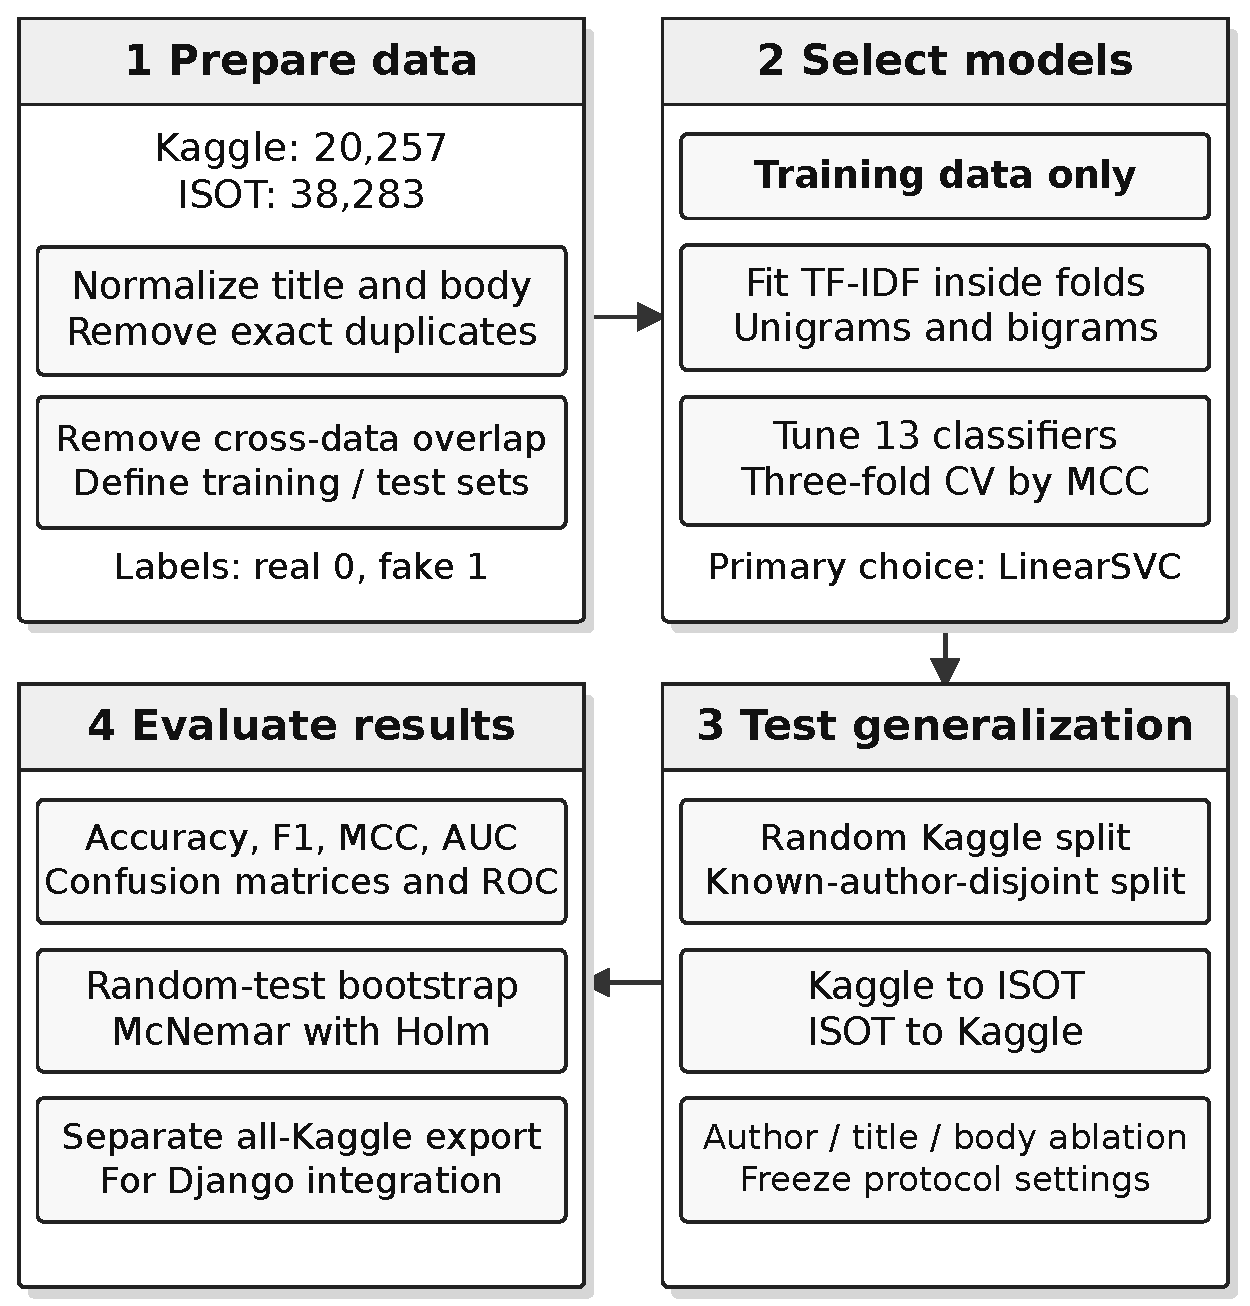
\includegraphics[width=\columnwidth]{figures/VeriFake_Figure_1.pdf}
\caption{VeriFake workflow. Each protocol fits features and selects settings using training data only. Forward transfer retains Kaggle training-CV settings. Intervals and paired tests use the random test; Algorithm~\ref{alg:eval} specifies the separate all-data export.}
\label{fig:workflow}
\end{figure}

\subsection{Text Representation and Classifiers}
The primary input concatenates normalized title, one space, and normalized body. TF-IDF uses word unigrams and bigrams, the scikit-learn English stop list, a minimum document frequency of 3, a maximum document proportion of 0.9, and at most 50,000 features. The default token rule retains tokens of at least two word characters. Values are stored in single precision. Let $f_{t,d}$ be the count of term $t$ in document $d$, $N$ the number of fitting documents, and $\mathrm{df}_t$ the number containing $t$. Sublinear term frequency and smoothed inverse document frequency give \cite{sklearn,tfidf}
\begin{equation}
 u_{t,d}=\begin{cases}(1+\ln f_{t,d})\left[\ln\frac{1+N}{1+\mathrm{df}_t}+1\right],&f_{t,d}>0,\\0,&f_{t,d}=0,\end{cases}
\label{eq:tfidf}
\end{equation}
followed by $x_d=u_d/\|u_d\|_2$ for nonzero vectors. A vector remains zero if no retained term occurs. All statistics in (\ref{eq:tfidf}) come from the applicable training fold or final training partition.

The thirteen classifiers are logistic regression (LR), multinomial and Bernoulli Naive Bayes (MNB and BNB), LinearSVC, radial-basis-function SVC (SVC-RBF), cosine-distance nearest neighbors (KNN), decision tree (DT), random forest (RF), extra trees (ET), AdaBoost, gradient boosting (GB), multilayer perceptron (MLP), and XGBoost (XGB). All use the same TF-IDF configuration. The candidate grids are given in Table~\ref{tab:grid}.

The linear support vector classifier uses $s(x)=w^\top x+b$ and predicts class 1 for $s(x)>0$. With $z_i=2y_i-1$, its L2-regularized squared-hinge formulation is \cite{liblinear}
\begin{equation}
\min_{w,b}\ \frac{1}{2}(\|w\|_2^2+b^2)+C\sum_i\max(0,1-z_i(w^\top x_i+b))^2.
\label{eq:svm}
\end{equation}
The intercept is implemented as a synthetic feature of value 1 and is regularized. We retain the implementation's automatic primal/dual solver choice, with a maximum of 5,000 iterations. The score is a margin, not a calibrated probability.

A classification tree selects splits by weighted reduction in Gini impurity, $G(v)=1-\sum_{c=0}^{1}p(c\mid v)^2$, where $p(c\mid v)$ is the class fraction at node $v$. RF averages the class probabilities produced by its $B$ trees \cite{breiman,sklearn}:
\begin{equation}
\widehat p(c\mid x)=B^{-1}\sum_{b=1}^{B}p_b(c\mid x),\qquad
\widehat y=\arg\max_{c\in\{0,1\}}\widehat p(c\mid x).
\label{eq:rf}
\end{equation}
RF uses bootstrap samples; ET uses randomized split thresholds without bootstrap sampling. Both have 300 trees. Thus the models solve classification problems; a regression mean-squared-error expression does not describe their evaluation here.

The MLP has one hidden layer with 128 rectified linear units and a sigmoid binary output. Its objective combines binary cross-entropy with an L2 weight penalty \cite{sklearn,mlp}:
\begin{equation}
\mathcal L=-\frac1n\sum_i[y_i\ln p_i+(1-y_i)\ln(1-p_i)]
+\frac{\alpha}{2n}\sum_\ell\|W_\ell\|_F^2.
\label{eq:mlp}
\end{equation}
Adam uses an initial learning rate of 0.001 and batches of 256. Training stops after at most 50 epochs, with 10\% of the fitting partition reserved for early stopping and a patience of three epochs. This internal stop uses validation accuracy. TF-IDF is fitted on the outer CV training fold before that internal subdivision, so this internal subset is not a fully isolated representation-validation split; the outer fold remains separate.

LR uses LIBLINEAR with at most 2,000 iterations. BNB binarizes nonzero TF-IDF entries using its default zero threshold. KNN uses distance weighting and brute-force cosine search. AdaBoost uses decision stumps. GB uses 300 depth-3 trees, a subsampling rate of 0.8, and a feature fraction of 0.1. XGB uses binary logistic loss, depth 6, learning rate 0.1, subsampling 0.8, column sampling 0.5, and CPU histogram training \cite{xgb}. Randomized estimators use seed 42.

\begin{table}[t]
\caption{Hyperparameter grids used separately within each tuning protocol. Other settings are fixed as described in Section III-C. None means no explicit depth limit.}
\label{tab:grid}\centering\small
\begin{tabular}{lp{5.7cm}}\toprule
Model & Candidate values\\\midrule
LR & $C\in\{1,10,100\}$\\
MNB, BNB & $\alpha\in\{0.01,0.1,1\}$\\
LinearSVC & $C\in\{0.1,1,10\}$\\
SVC-RBF & $C\in\{1,10\}$; $\gamma=\texttt{scale}$\\
KNN & Neighbors $\in\{5,15,31\}$\\
DT & Depth $\in\{\text{None},50\}$; leaf size $\in\{1,5\}$\\
RF, ET & Features $\in\{\texttt{sqrt},\texttt{log2}\}$; leaf size $\in\{1,2\}$\\
AdaBoost & Estimators $\in\{200,400\}$; rate $\in\{0.5,1\}$\\
GB & Learning rate $\in\{0.1,0.3\}$\\
MLP & $\alpha\in\{10^{-4},10^{-3}\}$\\
XGB & Estimators $\in\{300,600\}$\\\bottomrule
\end{tabular}
\end{table}

\subsection{Evaluation Algorithm and Measures}
Algorithm~\ref{alg:eval} specifies the training and reporting boundary illustrated in Fig.~\ref{fig:workflow}. It is a description of the implemented procedure, not a newly proposed learning algorithm. The ablation fits four models, LinearSVC, LR, MNB, and RF, on title only, author plus title, title plus body, and author plus title plus body. Hyperparameters selected for title plus body are frozen across input variants within each protocol. Therefore the comparison measures input sensitivity at those settings, rather than the best separately tuned performance of every variant.

\begin{figure}[t]
\centering\begin{minipage}{\columnwidth}
\hrule\vspace{3pt}\refstepcounter{algorithm}\textbf{Algorithm 1. Training-only selection and evaluation}\label{alg:eval}\vspace{3pt}\hrule
\begin{enumerate}[leftmargin=1.6em,itemsep=1pt,topsep=3pt,label=\arabic*.]\footnotesize
\item[]\textbf{Input:} Cleaned Kaggle $K$, cleaned ISOT $I$, grids $H_m$
\item Set seed 42; construct title-and-body input.
\item Split $K$ into stratified training $K_r$ and test $K_t$.
\item\textbf{For each classifier $m$:}
\item Search $H_m$ on $K_r$ with three-fold CV; fit a new TF-IDF inside each fold; maximize mean MCC.
\item Refit on $K_r$; save labels and scores on $K_t$.
\item\textbf{End for.}
\item Select family $m^*$ by training CV MCC only.
\item Exclude missing authors; form disjoint author groups.
\item Repeat selection within group training folds; evaluate the held-out groups for every classifier.
\item\textbf{For each classifier $m$:}
\item Refit on all $K$ with its $K_r$ settings; test on $I$.
\item Tune on $I$ only; refit on $I$; test on all $K$.
\item\textbf{End for.}
\item Fit input variants with protocol settings held fixed.
\item Compute metrics from saved labels and scores; calculate conditional intervals and paired tests on $K_t$.
\item Refit $m^*$ on all $K$ for a separate deployment export.
\item[]\textbf{Output:} Prediction records, tables, figures, and model export
\end{enumerate}\hrule
\end{minipage}
\end{figure}

Label 1 is the positive class. With true positives TP, true negatives TN, false positives FP, and false negatives FN, accuracy is $(\mathrm{TP}+\mathrm{TN})/n$, precision is $\mathrm{TP}/(\mathrm{TP}+\mathrm{FP})$, recall is $\mathrm{TP}/(\mathrm{TP}+\mathrm{FN})$, and F1 is $2\mathrm{TP}/(2\mathrm{TP}+\mathrm{FP}+\mathrm{FN})$. We also report MCC, which incorporates all four confusion counts \cite{chicco}:
\begin{equation}
\mathrm{MCC}=\frac{\mathrm{TP}\mathrm{TN}-\mathrm{FP}\mathrm{FN}}
{\sqrt{(\mathrm{TP}+\mathrm{FP})(\mathrm{TP}+\mathrm{FN})(\mathrm{TN}+\mathrm{FP})(\mathrm{TN}+\mathrm{FN})}}.
\label{eq:mcc}
\end{equation}
ROC-AUC uses positive-class probabilities when available and decision scores for the support vector classifiers. It never uses binary predictions as ranking scores. One thousand bootstrap resamples of the random test set give percentile 95\% intervals for accuracy and MCC. Exact two-sided McNemar tests compare the selected model against the other twelve classifiers, with Holm correction. These estimates condition on one fitted model and one outer split; they do not quantify variability over repeated training or new publishers.

\subsection{Implementation and Web Integration}
The experiments ran on the University of Wyoming ARCC MedicineBow system using Python 3.11.16, scikit-learn 1.9.1, XGBoost 3.2.0, NumPy 2.4.6, and SciPy 1.17.1. Grid search used eight workers within a 32-CPU allocation, with estimator thread counts restricted to avoid nested parallelism. The main comparison used CPU training. A separate XGB diagnostic used a training-only holdout to compare CPU and H100 GPU execution; this diagnostic did not select the primary backend from test results.

The Django prototype provides registration, login, and a form for news input. For integration, the exported pipeline accepts raw title, one space, and raw body, then applies normalization, fitted TF-IDF, and LinearSVC. The export is fitted on all cleaned Kaggle records after evaluation and must not be used to reproduce held-out scores. The recorded export check compared its labels with the fitted text pipeline on ten examples. This is a preprocessing consistency check, not a deployment or security audit. End-to-end web latency, user effectiveness, and updated live-server behavior were not evaluated.

The project repository is \url{https://github.com/mmrwyo/VeriFake}. Recorded acquisition mirrors are \nolinkurl{Shiv-Pal/Fake_Real_News} and \nolinkurl{koliskos/fake_news} on Hugging Face; Kaggle and ISOT remain the original sources. Checksums, split manifests, settings, and saved predictions document the run. The URL does not imply redistribution rights for news articles.

\begin{figure*}[t]
\centering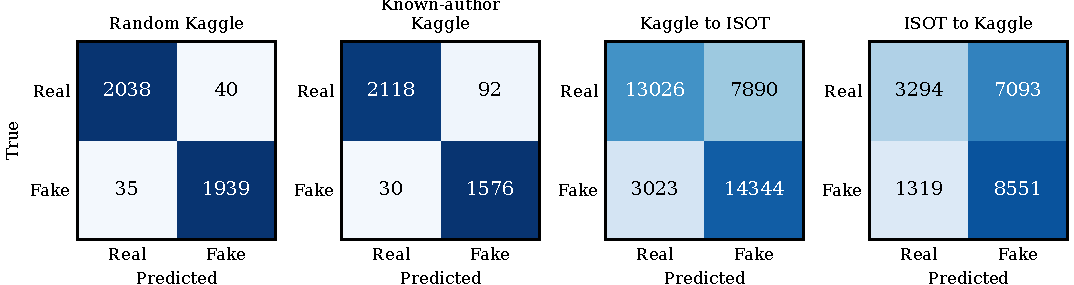
\includegraphics[width=\textwidth]{figures/confusion_row.pdf}
\caption{LinearSVC confusion matrices from saved predictions for the four title-and-body protocols. Rows are true labels and columns are predicted labels; fake is class 1. Printed values are article counts, while color is normalized within each true class. The family is selected by primary training CV MCC and fitted separately for each protocol.}
\label{fig:cm}
\end{figure*}

\section{Experimental Results}
\subsection{Comparison on the Random Split}
Table~\ref{tab:primary} reports all thirteen classifiers on the same 4,052 test articles. LinearSVC has the highest mean training CV MCC, 0.9607, with $C=10$. Its held-out accuracy is 98.15\%, F1 is 98.10\%, MCC is 0.9630, and ROC-AUC is 0.9977. LR has one fewer error and a slightly higher accuracy of 98.17\%, but its training CV MCC is lower at 0.9584. This difference illustrates why selecting the final family from test accuracy would change the stated selection rule.

\begin{table}[t]
\caption{Random-split results for title plus body on 4,052 Kaggle articles, ordered by training CV MCC. Acc., P, R, and F1 are percentages; MCC and AUC are unitless. P and R refer to fake articles.}
\label{tab:primary}\centering\footnotesize
\setlength{\tabcolsep}{3pt}
\begin{tabular}{lrrrrrrr}\toprule
Model & CV MCC & Acc. & P & R & F1 & MCC & AUC\\\midrule
LinearSVC & 0.9607 & 98.15 & 97.98 & 98.23 & 98.10 & 0.9630 & 0.9977\\
LR & 0.9584 & 98.17 & 98.03 & 98.23 & 98.13 & 0.9635 & 0.9977\\
XGB & 0.9577 & 97.75 & 97.10 & 98.33 & 97.71 & 0.9551 & 0.9976\\
SVC-RBF & 0.9537 & 97.90 & 97.68 & 98.02 & 97.85 & 0.9580 & 0.9975\\
AdaBoost & 0.9385 & 96.22 & 95.19 & 97.16 & 96.16 & 0.9247 & 0.9943\\
GB & 0.9375 & 96.59 & 95.45 & 97.67 & 96.54 & 0.9321 & 0.9934\\
MLP & 0.9369 & 97.46 & 97.42 & 97.37 & 97.39 & 0.9491 & 0.9968\\
RF & 0.9284 & 96.32 & 95.97 & 96.50 & 96.24 & 0.9264 & 0.9937\\
ET & 0.9215 & 96.13 & 96.57 & 95.44 & 96.00 & 0.9225 & 0.9945\\
DT & 0.8916 & 94.42 & 94.14 & 94.43 & 94.28 & 0.8884 & 0.9303\\
MNB & 0.8785 & 93.58 & 96.78 & 89.82 & 93.17 & 0.8735 & 0.9899\\
KNN & 0.8393 & 92.15 & 96.41 & 87.13 & 91.54 & 0.8463 & 0.9816\\
BNB & 0.7850 & 89.49 & 85.97 & 93.72 & 89.68 & 0.7931 & 0.9440\\
\bottomrule\end{tabular}\end{table}

The LinearSVC confusion counts are TN=2,038, FP=40, FN=35, and TP=1,939. Its accuracy interval is 97.73\% to 98.54\%, and its MCC interval is 0.9546 to 0.9709. The paired comparison with LR is not significant after correction ($p=1.000$); those with XGB and SVC-RBF also are not significant ($p=0.457$ for each). Failure to reject a difference does not demonstrate equivalence. The corrected comparisons favor LinearSVC over the remaining nine models at the 0.05 level.

RF and ET achieve 96.32\% and 96.13\% accuracy. XGB reaches 97.75\%, rather than the near-chance result of an earlier implementation. Separate training-only CPU and GPU diagnostics each reached 97.75\%, with exact agreement between their scikit-learn and DMatrix prediction interfaces. This does not establish the earlier failure's cause; the main comparison retains its prespecified CPU backend.

\subsection{Author Separation and Dataset Transfer}
Table~\ref{tab:general} summarizes LinearSVC across protocols. Known-author-disjoint accuracy is 96.80\% with $C=1$, versus 98.15\% on the random test. Different test populations and training samples prevent treating this difference as the isolated causal effect of author overlap.

\begin{table}[t]
\caption{LinearSVC across protocols using title plus body. Acc. is accuracy in percent. MCC and AUC are unitless; positive class is fake. Family selection uses primary training CV only.}
\label{tab:general}\centering\small
\begin{tabular}{lrrrr}\toprule
Test setting & Test $n$ & Acc. & MCC & AUC\\\midrule
Random Kaggle & 4,052 & 98.15 & 0.9630 & 0.9977\\
Known-author Kaggle & 3,816 & 96.80 & 0.9353 & 0.9971\\
Kaggle to ISOT & 38,283 & 71.49 & 0.4527 & 0.8144\\
ISOT to Kaggle & 20,257 & 58.47 & 0.2187 & 0.6652\\\bottomrule
\end{tabular}
\end{table}

Forward and reverse transfer accuracies fall to 71.49\% and 58.47\%, with MCC values of 0.4527 and 0.2187. Thus the loss is not explained merely by class proportions. Figures~\ref{fig:cm} and \ref{fig:roc} show class-specific errors and score discrimination.



Rankings change under transfer. MLP leads forward accuracy at 78.17\%, despite trailing LinearSVC on the random split. AdaBoost and RF lead reverse accuracy at 63.18\% and 63.16\%. These descriptive target-set comparisons do not change the primary model selected using training CV.

\subsection{Sensitivity to Author and Text Inputs}
Table~\ref{tab:ablation} reports the LinearSVC ablation. Title-only accuracy is 92.87\% on the random split and 91.12\% on the group split. Adding the body improves both. Author plus title yields the highest random-split accuracy, 99.56\%, but only 89.68\% under known-author separation. This pattern is consistent with dependence on author-related cues, although different test populations prevent a causal attribution to author overlap alone.

\begin{table}[t]
\caption{LinearSVC input ablation with hyperparameters frozen within each protocol. R is the random test ($n=4,052$), G the known-author-disjoint test ($n=3,816$). Accuracy is percent.}
\label{tab:ablation}\centering\small
\begin{tabular}{lrrrr}\toprule
Input & R Acc. & R MCC & G Acc. & G MCC\\\midrule
Title & 92.87 & 0.8576 & 91.12 & 0.8272\\
Author + title & 99.56 & 0.9911 & 89.68 & 0.8109\\
Title + body & 98.15 & 0.9630 & 96.80 & 0.9353\\
Author + title + body & 98.67 & 0.9733 & 97.20 & 0.9433\\\bottomrule
\end{tabular}
\end{table}

Metadata is not uniformly harmful: adding author to title plus body raises group accuracy from 96.80\% to 97.20\%. Author strings may share useful terms, while body text supplies additional signals. The narrower finding is that strong author-plus-title random performance does not transfer to unseen author groups. Primary inference uses title plus body without requiring authors.

\begin{figure}[t]
\centering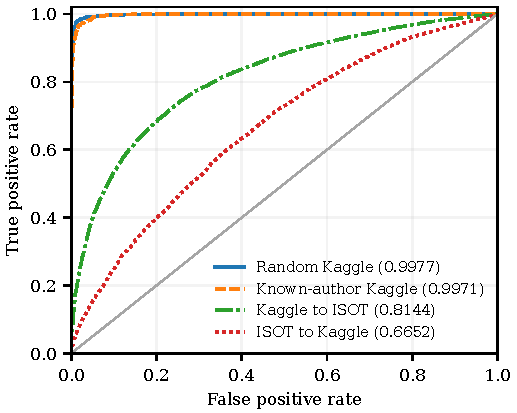
\includegraphics[width=\columnwidth]{figures/roc_selected.pdf}
\caption{LinearSVC ROC curves from continuous decision scores under the four title-and-body protocols. Fake is the positive class; legends report ROC-AUC. The gray diagonal denotes chance ranking. Curves describe score ordering, not probability calibration or factual verification.}
\label{fig:roc}
\end{figure}

\section{Discussion and Limitations}
Strong within-collection performance coexists with weak transfer. Topic distributions, collection rules, and source-dependent labels may explain this gap, but our experiments do not isolate their effects. The interpretation agrees with recent dataset-bias and generalization studies \cite{kishi,verhoeven}.

Exact matching misses paraphrases, syndicated variants, and related reports. Normalized author strings do not uniquely identify people or publishers, and excluding missing authors changes the group-test population. ISOT's Reuters-derived real class may retain source-style cues after marker removal. Transfer results apply to the filtered collections, not every original article.

Each within-collection protocol uses one outer split. Bootstrap intervals condition on that split and fitted model. Limited, unequal search grids and the MLP training budget constrain comparisons. Transformer baselines, temporal or publisher-disjoint tests, calibration, and human fact-checking outcomes were not evaluated. These limits preclude claims of state-of-the-art performance or readiness for autonomous moderation.

The interface should display a classifier output, not a probability of truth. Operational use requires integration and latency checks, user testing, and representative news-stream evaluation. Evidence retrieval and claim-level assessment are necessary for a factual-verification service.

\section{Conclusion}
VeriFake documents a thirteen-classifier comparison with training-only feature fitting. CV-selected LinearSVC reaches 98.15\% random-test accuracy, versus 71.49\% forward transfer and 58.47\% reverse transfer. The author-input ablation shows why near-perfect random results require qualification. The evaluation records and export support further development, while publisher separation, temporal testing, calibration, and evidence retrieval remain necessary for dependable deployment.

\section*{Acknowledgment}
OpenAI ChatGPT assisted with code preparation, figure-generation scripts, and the organization and wording of the abstract and Sections I-VI. The reported numerical results come from the recorded computational experiments. The authors are responsible for the final content.

\begin{thebibliography}{22}
\bibitem{kishi} Y. Kishi, Y. Arima, and H. Iyatomi, ``Fake news detection strategies under dataset bias: Using large-scale coarse-grained labels,'' in \emph{Proc. EACL, Student Research Workshop}, 2026, pp. 612-621, \href{https://doi.org/10.18653/v1/2026.eacl-srw.47}{doi: \nolinkurl{10.18653/v1/2026.eacl-srw.47}}.
\bibitem{verhoeven} I. Verhoeven, P. Mishra, and E. Shutova, ``Yesterday's news: Benchmarking multi-dimensional out-of-distribution generalization of misinformation detection models,'' \emph{Computational Linguistics}, vol. 52, no. 2, pp. 619-675, 2026, \href{https://doi.org/10.1162/coli.a.585}{doi: \nolinkurl{10.1162/coli.a.585}}.
\bibitem{zhou} X. Zhou and R. Zafarani, ``A survey of fake news: Fundamental theories, detection methods, and opportunities,'' \emph{ACM Computing Surveys}, vol. 53, no. 5, Art. no. 109, 2020, \href{https://doi.org/10.1145/3395046}{doi: \nolinkurl{10.1145/3395046}}.
\bibitem{ahmed} H. Ahmed, I. Traore, and S. Saad, ``Detecting opinion spams and fake news using text classification,'' \emph{Security and Privacy}, vol. 1, no. 1, Art. no. e9, 2018, \href{https://doi.org/10.1002/spy2.9}{doi: \nolinkurl{10.1002/spy2.9}}.
\bibitem{liar} W. Y. Wang, ```Liar, Liar Pants on Fire': A new benchmark dataset for fake news detection,'' in \emph{Proc. ACL}, vol. 2, 2017, pp. 422-426, \href{https://doi.org/10.18653/v1/P17-2067}{doi: \nolinkurl{10.18653/v1/P17-2067}}.
\bibitem{fakenewsnet} K. Shu, D. Mahudeswaran, S. Wang, D. Lee, and H. Liu, ``FakeNewsNet: A data repository with news content, social context, and spatiotemporal information for studying fake news on social media,'' \emph{Big Data}, vol. 8, no. 3, pp. 171-188, 2020, \href{https://doi.org/10.1089/big.2020.0062}{doi: \nolinkurl{10.1089/big.2020.0062}}.
\bibitem{fever} J. Thorne, A. Vlachos, C. Christodoulopoulos, and A. Mittal, ``FEVER: A large-scale dataset for fact extraction and verification,'' in \emph{Proc. NAACL-HLT}, vol. 1, 2018, pp. 809-819, \href{https://doi.org/10.18653/v1/N18-1074}{doi: \nolinkurl{10.18653/v1/N18-1074}}.
\bibitem{teller} H. Liu, W. Wang, H. Li, and H. Li, ``TELLER: A trustworthy framework for explainable, generalizable and controllable fake news detection,'' in \emph{Findings of ACL}, 2024, pp. 15556-15583, \href{https://doi.org/10.18653/v1/2024.findings-acl.919}{doi: \nolinkurl{10.18653/v1/2024.findings-acl.919}}.
\bibitem{ma} X. Ma, Y. Zhang, K. Ding, J. Yang, J. Wu, and H. Fan, ``On fake news detection with LLM enhanced semantics mining,'' in \emph{Proc. EMNLP}, 2024, pp. 508-521, \href{https://doi.org/10.18653/v1/2024.emnlp-main.31}{doi: \nolinkurl{10.18653/v1/2024.emnlp-main.31}}.
\bibitem{wei} W. Wei, Y. Zhang, J. Li, P. Liu, and D. Zhou, ``Cross-domain fake news detection based on dual-granularity adversarial training,'' in \emph{Proc. COLING}, 2025, pp. 9407-9417. [Online]. Available: \url{https://aclanthology.org/2025.coling-main.631/}
\bibitem{su} J. Su, C. Cardie, and P. Nakov, ``Adapting fake news detection to the era of large language models,'' in \emph{Findings of NAACL}, 2024, pp. 1473-1490, \href{https://doi.org/10.18653/v1/2024.findings-naacl.95}{doi: \nolinkurl{10.18653/v1/2024.findings-naacl.95}}.
\bibitem{triplefact} C. Xu and N. Yan, ``TripleFact: Defending data contamination in the evaluation of LLM-driven fake news detection,'' in \emph{Proc. ACL}, vol. 1, 2025, pp. 8808-8823, \href{https://doi.org/10.18653/v1/2025.acl-long.431}{doi: \nolinkurl{10.18653/v1/2025.acl-long.431}}.
\bibitem{kapoor} S. Kapoor and A. Narayanan, ``Leakage and the reproducibility crisis in machine-learning-based science,'' \emph{Patterns}, vol. 4, no. 9, Art. no. 100804, 2023, \href{https://doi.org/10.1016/j.patter.2023.100804}{doi: \nolinkurl{10.1016/j.patter.2023.100804}}.
\bibitem{kaggle} Kaggle, ``Fake News,'' competition dataset. [Online]. Available: \url{https://www.kaggle.com/competitions/fake-news}
\bibitem{isot} ISOT Research Lab, University of Victoria, ``ISOT Fake News Dataset,'' dataset documentation. [Online]. Available: \url{https://onlineacademiccommunity.uvic.ca/isot/datasets/}
\bibitem{sklearn} F. Pedregosa \emph{et al.}, ``Scikit-learn: Machine learning in Python,'' \emph{Journal of Machine Learning Research}, vol. 12, pp. 2825-2830, 2011. [Online]. Available: \url{https://jmlr.org/papers/v12/pedregosa11a.html}
\bibitem{tfidf} Scikit-learn developers, ``Feature extraction,'' scikit-learn 1.9.1 documentation, 2026. [Online]. Available: \url{https://scikit-learn.org/stable/modules/feature_extraction.html}
\bibitem{liblinear} R.-E. Fan, K.-W. Chang, C.-J. Hsieh, X.-R. Wang, and C.-J. Lin, ``LIBLINEAR: A library for large linear classification,'' \emph{Journal of Machine Learning Research}, vol. 9, pp. 1871-1874, 2008. [Online]. Available: \url{https://jmlr.org/papers/v9/fan08a.html}
\bibitem{breiman} L. Breiman, ``Random forests,'' \emph{Machine Learning}, vol. 45, pp. 5-32, 2001, \href{https://doi.org/10.1023/A:1010933404324}{doi: \nolinkurl{10.1023/A:1010933404324}}.
\bibitem{mlp} Scikit-learn developers, ``Neural network models (supervised),'' scikit-learn 1.9.1 documentation, 2026. [Online]. Available: \url{https://scikit-learn.org/stable/modules/neural_networks_supervised.html}
\bibitem{xgb} T. Chen and C. Guestrin, ``XGBoost: A scalable tree boosting system,'' in \emph{Proc. ACM SIGKDD}, 2016, pp. 785-794, \href{https://doi.org/10.1145/2939672.2939785}{doi: \nolinkurl{10.1145/2939672.2939785}}.
\bibitem{chicco} D. Chicco and G. Jurman, ``The advantages of the Matthews correlation coefficient (MCC) over F1 score and accuracy in binary classification evaluation,'' \emph{BMC Genomics}, vol. 21, Art. no. 6, 2020, \href{https://doi.org/10.1186/s12864-019-6413-7}{doi: \nolinkurl{10.1186/s12864-019-6413-7}}.
\end{thebibliography}
\end{document}
